\section{Data}
% 
% 
\subsection{Introduction to Match Data Set}
\paragraph{Our dataset includes full-season data from 2007 to 2022 and partial-season English Premier League (EPL) match data up to December 7, 2023, for the 2023-2024 season. The data is organized into CSV files, each titled with the respective season "20xx-20xy". Each file contains match records for various teams.}
\begin{enumerate}
    \item \textbf{Matches Played (MP):} Represents the number of matches in which the team participated in the current season.
    % 
    \item \textbf{Wins (W):} Indicates the number of victories the team achieved in the current season. In a match, winning refers to having a higher goal count than the opponent at the end of the game.
    % 
    \item \textbf{Draws (D):} Represents the number of matches in which the team ended with a tied score. In a match, a draw occurs when both teams have an equal number of goals at the end.
    % 
    \item \textbf{Losses (L):} Indicates the number of matches in which the team was defeated in the current season. In a match, losing refers to having fewer goals than the opponent at the end.
    % 
    \item \textbf{Goals For (GF):} Represents the total number of goals scored by the team in the current season. This is an indicator reflecting the team's offensive strength.
    % 
    \item \textbf{Goals Against (GA):} Represents the total number of goals conceded by the team in the current season. This is an indicator reflecting the team's defensive capabilities.
    % 
    \item \textbf{Goals Difference (GD):} Represents the difference between the number of goals scored and the number of goals conceded by the team in the current season. It is calculated as Goals For - Goals Against. A positive value indicates that the team's offensive strength is greater than its defensive strength, while a negative value indicates the opposite.
    % 
    \item \textbf{Points (Pts):} Represents the cumulative points earned by the team in the current season. Typically, a win awards the team 3 points, a draw awards 1 point, and a loss awards no points. Points are a crucial metric for assessing the overall competitive level of the team and are commonly used to determine team rankings in leagues.
\end{enumerate}
\paragraph{These variables provide quantitative measures of various aspects of the team's performance in the current season, including match count, win-loss-draw record, offensive and defensive performance, and overall competitiveness assessed through point accumulation. These indicators are common and important metrics in football analysis.}
% 
% 
% 
\begin{center}
\begin{table}
    \caption{Example Dataset: 2014\_15.csv}
    \begin{tabular}{lcccccccc}
        \toprule
        \textbf{Team} & \textbf{MP} & \textbf{Win} & \textbf{Draw} & \textbf{Loss} & \textbf{GF} & \textbf{GA} & \textbf{GD} & \textbf{Points} \\
        \midrule
        Chelsea FC & 38 & 26 & 9 & 3 & 73 & 32 & 41 & 87 \\
        Manchester City FC & 38 & 24 & 7 & 7 & 83 & 38 & 45 & 79 \\
        Arsenal FC & 38 & 22 & 9 & 7 & 71 & 36 & 35 & 75 \\
        Manchester United FC & 38 & 20 & 10 & 8 & 62 & 37 & 25 & 70 \\
        Tottenham Hotspur FC & 38 & 19 & 7 & 12 & 58 & 53 & 5 & 64 \\
        Liverpool FC & 38 & 18 & 8 & 12 & 52 & 48 & 4 & 62 \\
        ... & ... & ... & ... & ... & ... & ... & ... & ... \\
        \bottomrule
    \end{tabular}
\end{table}
\end{center}
% 
% 
\subsection{Data Acquisition Framework}
% 
\paragraph{Instead of using the open source data set, in order to obtain up-to-date and customized data, we wrote Python scripts to grab data from the web.}
\paragraph{Due to the modern structure of websites relying on user interaction for dynamic data retrieval, traditional Python web scraping libraries like requests face challenges in obtaining specific data. Therefore, we employ Selenium, a web automation testing framework. Selenium allows us to simulate human interaction by opening a browser on a computer, navigating to a website, and interacting with elements such as buttons. This assists us in navigating to the desired season page on the website. Subsequently, we use Python to parse the HTML content, extract the data mentioned earlier, and finally, employ the Pandas library to save the acquired data to a CSV file.}
% 
% 
% 
% 
\begin{figure}[H]
    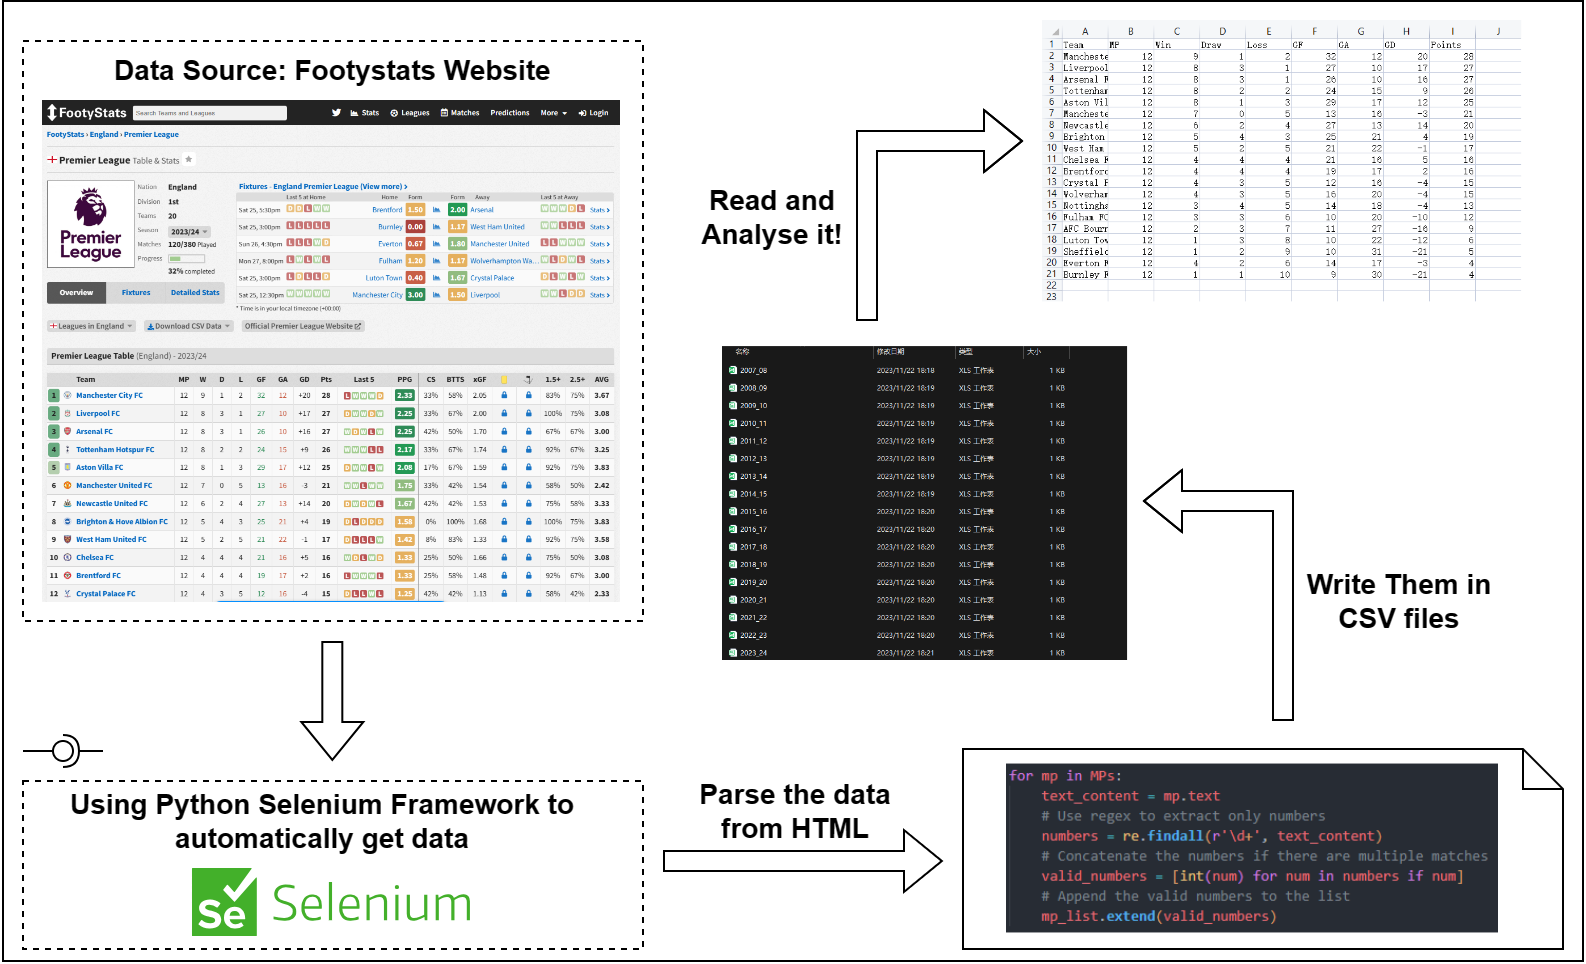
\includegraphics[width=\textwidth]{pic/DataGrab.png}
    \caption{Flow Chart for Data Grabbing}
    % \label{fig:DataGrab}
\end{figure}
% \paragraph{}
% 
% 
% 
\paragraph{We put the data acquisition part code in the Appnedix Section (\ref{sec:GetData}).}
% 
% 
% 
% 